\chapter{Wires, Crosstalk and Signals Between Chips}
\label{ch:wires}

Transistors get the attention, but a modern chip contains tens of kilometers of wire, stacked in a dozen or more layers. Wires set much of a chip's speed and power, and they interfere with each other. This chapter covers on-chip wiring, crosstalk, how signals travel between chips, and the bandwidth calculations that come up in assessment questions.

\section{The metal stack}

Above the transistors sits a stack of metal layers separated by insulating material (Figure~\ref{fig:metalstack}). Vertical connections between layers are called \term{vias}.

\begin{figure}[h]
\centering
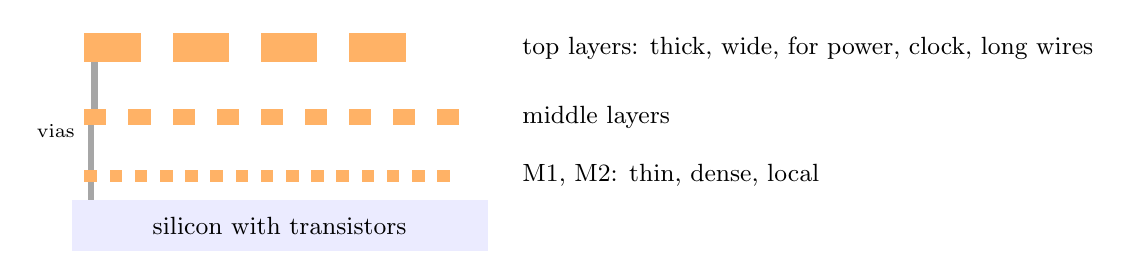
\begin{tikzpicture}[scale=0.8]
  \fill[blue!8] (0,0) rectangle (6.6,0.8); \node at (3.3,0.4) {\small silicon with transistors};
  \foreach \x in {0.2,0.6,...,6.2} \fill[orange!60] (\x,1.1) rectangle (\x+0.2,1.28);
  \foreach \x in {0.2,0.9,...,6.1} \fill[orange!60] (\x,2.0) rectangle (\x+0.35,2.25);
  \foreach \x in {0.2,1.6,...,5.8} \fill[orange!60] (\x,3.0) rectangle (\x+0.9,3.45);
  \fill[gray!70] (0.25,0.8) rectangle (0.35,1.1);
  \fill[gray!70] (0.25,1.28) rectangle (0.35,2.0);
  \fill[gray!70] (0.3,2.25) rectangle (0.42,3.0);
  \node[left,font=\scriptsize] at (0.2,1.9) {vias};
  \node[anchor=west,font=\small] at (7.0,1.2) {M1, M2: thin, dense, local};
  \node[anchor=west,font=\small] at (7.0,2.12) {middle layers};
  \node[anchor=west,font=\small] at (7.0,3.22) {top layers: thick, wide, for power, clock, long wires};
\end{tikzpicture}
\caption{Wiring layers above the transistors (not to scale). Lower layers are thin and closely packed; upper layers are thick and widely spaced.}
\label{fig:metalstack}
\end{figure}

\begin{itemize}
  \item The \textbf{lowest layers} are thin and densely packed, for short connections between nearby transistors.
  \item The \textbf{highest layers} are thick and wide. They carry power, ground, the clock, and long signals that cross the chip, because thick wires have much lower resistance.
  \item Modern chips use \textbf{copper} wires (lower resistivity than aluminum, and more resistant to electromigration), embedded in \textbf{low-$k$} insulators that reduce capacitance between wires.
\end{itemize}

\section{Wire resistance}

A wire's resistance is $R = \rho L/(W T)$, with length $L$, width $W$ and thickness $T$. Since all wires on one layer have the same thickness, designers use the layer's \term{sheet resistance} $R_\square = \rho/T$, in ohms per square. A wire's resistance is then its sheet resistance times the number of \emph{squares} it contains, length divided by width:
\[
  R = R_\square \cdot \frac{L}{W}.
\]
(A square of any size has the same resistance: a bigger square is longer, but proportionally wider.)

\begin{worked}{resistance of a thin wire}
A wire on a lower layer is 1\,mm long and 50\,nm wide, with a sheet resistance of 0.2\,$\Omega/\square$.
Squares: $10^{-3}/(50\times10^{-9}) = 20{,}000$. Resistance: $0.2 \times 20{,}000 = 4$\,k$\Omega$, comparable to a transistor's resistance. Long thin wires are slow.
\end{worked}

At these tiny dimensions, copper's effective resistivity is also higher than in bulk copper, because electrons scatter off the wire's surfaces and grain boundaries, and part of the cross-section is taken up by a barrier liner. Wire resistance is one of the hardest problems in advanced chips.

\section{Wire capacitance and crosstalk}

A wire has capacitance to the layers above and below (effectively to ground) and to its \emph{neighbors} on the same layer. In dense wiring, neighbor capacitance, called \term{coupling capacitance}, is often the largest part. Coupling causes \term{crosstalk}: a switching wire (the \term{aggressor}) disturbs a nearby wire (the \term{victim}).

\paragraph{Noise on a quiet victim.} If the victim is supposed to hold steady, a switching aggressor pushes charge onto it through the coupling capacitance $C_c$. If the victim's driver did not fight back at all, the victim's voltage would jump by
\[
  \Delta V \approx \VDD\,\frac{C_c}{C_c + C_g},
\]
where $C_g$ is the victim's capacitance to ground. A real driver pulls it back, so the result is a glitch. A large enough glitch can flip a latch or a dynamic node.

\begin{worked}{size of a crosstalk glitch}
$C_c = 10$\,fF, $C_g = 30$\,fF, $\VDD = 0.8$\,V. Worst case: $\Delta V \approx 0.8 \times 10/40 = 0.2$\,V, a quarter of the supply.
\end{worked}

\paragraph{Delay change on a switching victim.} If both wires switch at once:
\begin{itemize}
  \item In \textbf{opposite} directions, the voltage across $C_c$ changes by $2\VDD$, so it acts like $2C_c$ (the Miller effect, Chapter~\ref{ch:delay}): the victim is \emph{slower}.
  \item In the \textbf{same} direction, the voltage across $C_c$ barely changes, so it acts like almost nothing: the victim is \emph{faster}.
\end{itemize}

\paragraph{Switching windows.} Crosstalk only matters if the aggressor switches while the victim is vulnerable. Each net has a \term{switching window}: the interval between the earliest and latest times it can change, found by adding up the shortest and longest delays along the paths that drive it. Two coupled nets can interact only where their windows overlap.

\begin{worked}{do these nets interact?}
Net A can switch anywhere from 1.0\,ns to 1.6\,ns after the clock edge. Net B, which runs next to it, can switch from 1.4\,ns to 2.2\,ns. Their windows overlap from 1.4\,ns to 1.6\,ns, so crosstalk is possible only in that interval. If B's window were 1.8 to 2.2\,ns, there would be no overlap and no timing crosstalk.
\end{worked}

\begin{onoa}
A reported question gives two adjacent nets driven by gates with known delays and asks during what window crosstalk might occur. Compute each net's earliest and latest switching times from its gate delays, then intersect the two intervals.
\end{onoa}

\paragraph{Fixes for crosstalk.} Increase the spacing between wires; put a grounded \term{shield} wire between sensitive wires; route neighbors on different layers or perpendicular to each other; make the victim's driver stronger; or insert buffers to shorten the coupled length.

\section{Signals between chips}

Off the chip, signals travel through package pins, circuit-board traces and connectors. At modern speeds these are transmission lines (Section~\ref{sec:tline}): signals travel as waves, reflections must be prevented by matching impedances and terminating lines, and losses in the board material smear fast edges.

\paragraph{Differential signaling.} Most fast links send each signal on \emph{two} wires carrying opposite voltages, and the receiver looks only at the \emph{difference}. Noise that hits both wires equally (common-mode noise) cancels out. Differential links can therefore use small voltage swings, which saves power and allows very high speeds. PCIe, USB, HDMI, Ethernet and NVIDIA's NVLink all use differential pairs.

\paragraph{SerDes.} Instead of many slow parallel wires that must stay perfectly aligned in time, high-speed links use a few very fast serial lanes. A \term{serializer/deserializer} (SerDes) converts wide parallel data into a fast bit stream and back. The receiver recovers the clock from the data's transitions, so the data is \term{encoded} to guarantee enough transitions: 8b/10b encoding (8 data bits sent as 10, 80\% efficient) or 128b/130b (about 98.5\% efficient).

\paragraph{Eye diagrams.} Engineers check link quality by overlaying many bit periods of the received signal. A clean link shows a wide-open ``eye'' between the 0 and 1 levels; noise, jitter and reflections close it.

\section{Bandwidth calculations}
\label{sec:bandwidth}

Bandwidth questions are mostly careful unit-keeping:
\[
  \text{bandwidth (bytes/s)} = \frac{\text{bus width (bits)} \times \text{transfers per second}}{8} \times \text{efficiency}.
\]

\begin{itemize}
  \item \textbf{DDR} (double data rate) transfers data on both the rising and falling clock edges: two transfers per clock cycle.
  \item Link speeds are often given in \textbf{GT/s} (giga-transfers per second), which for a single lane equals Gb/s before encoding overhead.
  \item Divide bits by 8 for bytes. Apply encoding efficiency and protocol overhead (packet headers) if the question includes them.
\end{itemize}

\begin{worked}{DDR bandwidth}
An 8-bit DDR interface has a 10\,GHz clock. Transfers per second: $2 \times 10^{10}$. Bandwidth: $8 \times 2\times10^{10}/8 = 2\times10^{10}$\,bytes/s $= 20$\,GB/s.

If instead ``10\,GHz'' were the data rate (10\,GT/s, already counting both edges), the answer would be 10\,GB/s. Read carefully which one a question means.
\end{worked}

\begin{worked}{memory and link bandwidth}
\textbf{HBM}: one stack has a 1024-bit interface at 6.4\,Gb/s per pin: $1024 \times 6.4/8 \approx 819$\,GB/s.

\textbf{PCIe}: a 16-lane link at 16\,GT/s per lane with 128b/130b encoding: $16 \times 16 \times (128/130)/8 \approx 31.5$\,GB/s in each direction.

\textbf{Protocol overhead}: if every 256-byte payload travels with 24 bytes of headers, only $256/280 \approx 91\%$ of the link carries data, so the payload rate is 91\% of the raw rate.
\end{worked}

\section{Packets and address alignment}

Links such as PCIe move data in \term{packets} with a maximum payload size. Memory systems also prefer requests that do not cross certain \term{aligned} boundaries (addresses that are multiples of 64 bytes, for example). A large read is therefore split into several reply packets, and the first packet may be short so that later packets start on aligned boundaries.

\begin{worked}{how many reply packets?}
A device reads 202 bytes starting at address \code{0x31121133}. Replies carry at most 64 bytes and must not cross a 64-byte-aligned boundary.

The address's offset within its 64-byte block is its low 6 bits: \code{0x33} $= 51$. The first packet can carry only up to the next boundary: $64 - 51 = 13$ bytes. Remaining: $202 - 13 = 189$ bytes, which takes $\lceil 189/64 \rceil = 3$ more packets (64, 64 and 61 bytes). Total: \textbf{4 packets}.

Here the simple estimate $\lceil 202/64 \rceil = 4$ happens to agree, but not always. A 128-byte read starting at offset 32 needs \emph{three} packets (32, 64, 32), not two.
\end{worked}

\begin{onoa}
A reported question asked for the number of completion packets for a 202-byte read at address \code{0x31121133} with a 64-byte maximum payload. The method above, with alignment, gives 4.
\end{onoa}

\section{Summary}

\begin{itemize}
  \item Lower metal layers are thin and dense; upper layers are thick, for power, clock and long wires.
  \item $R = R_\square \cdot L/W$; very thin wires are surprisingly resistive.
  \item Coupling capacitance causes crosstalk: glitches on quiet victims ($\Delta V \approx \VDD C_c/(C_c+C_g)$) and delay changes on switching ones (opposite directions slower, same direction faster).
  \item Crosstalk needs overlapping switching windows.
  \item Fast chip-to-chip links are differential, serial (SerDes) and encoded.
  \item Bandwidth $=$ width $\times$ transfer rate $/ 8 \times$ efficiency; DDR doubles transfers per clock.
  \item Reads are split into packets at the maximum payload size and at aligned boundaries.
\end{itemize}

\section{Exercises}

\begin{enumerate}
  \item A wire is 200\,$\mu$m long and 0.1\,$\mu$m wide, on a layer with $R_\square = 0.1\,\Omega/\square$. What is its resistance?
  \item $C_c = 5$\,fF, $C_g = 15$\,fF, $\VDD = 0.8$\,V. Estimate the worst-case crosstalk glitch.
  \item Net A switches between 0.2 and 0.5\,ns; net B between 0.6 and 0.9\,ns. Can they cause timing crosstalk?
  \item How does a neighbor switching in the opposite direction affect a victim's delay? In the same direction?
  \item A 32-bit DDR bus runs at a 1.6\,GHz clock. What is its bandwidth?
  \item A PCIe link has 8 lanes at 8\,GT/s with 128b/130b encoding. What is its bandwidth per direction?
  \item A device reads 100 bytes starting at address \code{0x1030}, with 64-byte maximum payloads that cannot cross 64-byte boundaries. How many packets?
  \item Why does differential signaling resist noise?
\end{enumerate}

\subsection*{Answers}
\begin{enumerate}
  \item $2000$ squares $\times\, 0.1 = 200\,\Omega$.
  \item $0.8 \times 5/20 = 0.2$\,V.
  \item No; their windows do not overlap.
  \item Opposite: slower (the coupling acts like double the capacitance). Same: faster.
  \item $32 \times 3.2\times10^9 / 8 = 12.8$\,GB/s.
  \item $8 \times 8 \times (128/130)/8 \approx 7.9$\,GB/s.
  \item Offset of \code{0x1030} in its 64-byte block is \code{0x30} $= 48$, so the first packet carries 16 bytes; the remaining 84 bytes need 2 more (64 and 20). Total 3 packets.
  \item Noise usually couples equally onto both wires of the pair, and the receiver only looks at the difference between them, so the common noise cancels.
\end{enumerate}
